\section{Establishing Body Movement Patterns as Behavioral Biometrics}\label{sec:learning}

\subsection{Preliminary Results}
In our preliminary study, we used Google glass to collect accelerometer data ($ACC$ in short) when a user moves her head with music, and studied whether head movement patterns are distinctive and repeatable. After collecting raw $ACC$ data samples, we went through the following steps to process the data:

\begin{enumerate}
\item \emph{Filtering}: Since the frequency spectrum of the $ACC$ samples is significantly concentrated within 5Hz, we filtered the raw samples using a low-pass digital Butterworth filter~\cite{challis1983design} by adopting a relaxed cut-off frequency of 10Hz. In this way, we removed spurious head movements and obtained smooth $ACC$ data.

\item \emph{Training Set Construction:} We constructed the training set to include $m$ $ACC$ samples from the legitimate user (which we refer to as \emph{true} $ACC$ samples), as well as $m$ $ACC$ samples each from $N$ random users (referred to as \emph{false} samples).

\item \emph{Signature Generation}: Next, we generated signatures from the filtered $ACC$ samples using the dynamic-time warping (DTW) tool~\cite{***}. DTW is generally used as a similarity matching tool for time-domain analysis of temporally varying signals. DTW compares a temporal signal with a reference signal over a certain time-window and yields a distance measure as the score. A low score (distance) implies that the test signal is in close match with the reference.

    Using DTW, we calculated the distances between true $ACC$ samples and the distances between true samples and false samples, and refer to these two types of signatures as same-user distance signatures as well as across-user distance signatures.

\item \emph{SVM Classification:} In the classification phase, we first calculated the DTW distances between the test sample and the true samples, and then feed these values and the signatures to a Support Vector Machine (SVM) for classification. SVM returns '1' to denote that the test user is legitimate and '0' to denote otherwise.

\end{enumerate}


\begin{table}[b]
\small
\begin{tabular}{|l||l|l|l||l|l|l||l|l|l||l|l|l|}\hline
& \multicolumn{3}{|c||}{2}& \multicolumn{3}{|c||}{3}& \multicolumn{3}{|c||}{6}& \multicolumn{3}{|c|}{10}\\\cline{2-13}
Sample duration (s)& FRR & FAR & BAC & FRR & FAR & BAC & FRR & FAR & BAC & FRR & FAR & BAC\\
&(\%) &(\%) &(\%) &(\%) &(\%) &(\%) &(\%) &(\%) &(\%) &(\%) &(\%) &(\%)\\\hline

SVM          & 25.0 & 16.74 &79.12 & 15.0 & 14.05 & 85.47 & 3.33& 6.66& 95.0  & 0.0& 9.62& 95.18\\\hline

\end{tabular}
\caption{Average FAR, FRR, and BAC for SVM-based classification when we choose different 4 imitators in the training set (from the total 15 imitators). We have the results for different sample durations. In these results, we use the earliest 40 owner samples in the training set.\label{tab:kfoldfalse-svm}}
\end{table}


\vspace{4pt}\textbf{Distinctiveness:} We designed the first set of experiments to show that even the simplest head movements are distinctive -- i.e., it is hard to imitate other's head movements. In this set of experiments, we employed simplest head movement patterns: nodding. We have one owner for the Google glass who designed the nodding pattern and 15 imitators who imitated the movement. We collected 100 10-second $ACC$ samples from the owner, during the course of 60 days (from 10/1/2014 to 11/30/2014), ensuring the owner's sensor data includes sufficient variation that naturally occurs with time. We also made a great deal of effort to make sure the imitators accurately imitate the owner's movement -- the owner carefully explained his movement pattern to each imitator, and sat through each data collection session for all the 15 imitators to make sure their movement pattern looks the same to the owner's eye. For each imitator, we collected 40 10-second $ACC$ samples. Using different combinations of training data and test data, we generated the classification results and summarized the mean FAR (false acceptance rate), FRR (false rejection rate), and BAC (balanced accuracy) in Table~\ref{tab:kfoldfalse-svm}. The results show that \emph{even simple nodding is not easy to imitate: nodding for 6 seconds can classify 95\% of the users.} %As the sample duration increases from 2 seconds to 6 seconds, the classification accuracy improves significantly -- the BAC value changes from 79.12\% to 95\% for top 1 testing, and from 87.95\% to 93.27\% for top 3 voting. After the sample duration reaches 6 seconds, the improvement becomes less pronounced. This suggests that a sample duration of 6 seconds is sufficient to successfully classify 95\% of the users. We feel that moving our head gently along with music for 6 seconds is in general not a cumbersome process for most users. It further suggests that even simple nodding is hard to imitate by others, and thus head-movement has the potential to %serve as a reliable biometric characteristic for smart wearable authentication.

\begin{figure*}[t]
\centering
\includegraphics [width=.85\linewidth]{../mobisys_paper/fig/exp2_frr_far_bac.pdf}
\caption{In this set of experiments, we studied whether a user can successfully repeat her own head-movement pattern. We had 8 subjects, each performing her own choice of head-movement patterns. We collected 38 samples for each subject. (a) shows the FRR and FAR results for each subject, and (b) shows the BAC results. Thresholding-based classification with top 3 voting was used to generate these results. \label{fig:exp2_frr_far_bac}}
\end{figure*}

\vspace{4pt}\textbf{Repeatability:} We designed the second set of experiments to show that a user can successfully repeat her own head movement if each user is asked to come up with their own movement patterns. In this set of experiments, we had 8 subjects, and for each subject, we collected 38 $ACC$ samples with sample duration of 10 seconds. Each subject performed different head-movement patterns of their choice. We report the average FAR, FRR, and BAC values in Figure~\ref{fig:exp2_frr_far_bac}, where Figure~\ref{fig:exp2_frr_far_bac}(a) shows the FRR and FAR values, while Figure~\ref{fig:exp2_frr_far_bac}(b) shows the BAC values. The results show that \emph{head-movements are highly repeatable.} Among the 8 subjects that we studied, the highest BAC value is 100\%, and the lowest is 91.81\%, with the average BAC value of 95.57\%.

%Overall, our preliminary results suggest that the head movement pattern is a very promising biometric candidate for wearable user authentication.

\subsection{Proposed Research}
Our preliminary results show that head movement patterns have the potential to be used as a reliable biometric characteristic for wearable user authentication. However, in order to develop a full-fledged authentication system using unique body movements, we need to address several important challenges.

\subsubsection{Feature Selection and Information Entropy}\label{sec:feature}
We usually characterize a person's body movements using accelerometer (ACC) signals and gyroscope (GYRO) signals that are a few seconds long. In this project, we will investigate the following statistical features that have been proposed for ACC/GYRO signals in the literature~\cite{palmerini2011feature,Pirttikangas2006feature,preece2009comparison,bao2004activity,zhang2011feature}: (1) mean, standard deviation, median, 25\%, and 75\% of frequency (in the frequency domain), (2) mean low and mean rectified high pass filtered signals (in the frequency space), (3) centroid frequency (in the frequency domain), (4) frequency dispersion (in the frequency domain), (5) power spectrum of entropy in acceleration/rotation and average energy in acceleration/rotation (in the frequency domain), (6) magnitude of first five components of FFT analysis (in the frequency domain), (6) jerk index that indicates the smoothness of the signal (in the time domain), (7) mean crossing (in the time domain), (8) maximum difference acceleration (in the time domain), (9) correlations between axes (in the time domain).

\vspace{4pt}\textbf{Boosting Information Entropy:} It is important to encode as much information as possible into the measured sensor signals, i.e., boosting information entropy. One way of achieving this goal is to have the user make movements following the external music stimuli -- different people translate music stimuli to motor movements in different ways. As a result, in addition to the above basic $ACC$/$GYRO$ features, we will also consider features concerned with the temporal relationship between music beats and corresponding body movements, such as mean and standard deviation of the interval values (between a music beat and the subsequent body movement), the top interval values, etc. These features show a person's motor response levels to external music stimuli.

In order to further boost the information entropy, we can even change the music track between a data collection session, so that we cannot only measure the user's response to music stimuli in a steady state, but we can also measure how fast the user adapts to the change of rhythm in the music. Therefore, given the same total sample duration, this method can pack more information to the resulting signals.



\subsubsection{Robust Authentication in Mobile Settings}
Our preliminary results show that head movements are rather distinctive and repeatable in very controlled settings -- all the data were collected when the participant was in a stationary setting, e.g., sitting on a chair. However, in reality, the behavior of body movement signatures over chaotic settings will be a key factor to decide on the effectiveness of this approach. %Our work only evaluates the case when a
%user is in a stationary setting when attempting to login, such as when sitting
%on the chair or standing still. The performance of this approach in realistic

\vspace{4pt}\textbf{Authenticating Walking Users:} In particular, we need to solve the challenge when the user is in a mobile context such as walking. In such a case, we can't rely on the original training data that is collected when the user was sitting or standing still any more; performing head/hand movements while walking will definitely lead to different movement signatures.

We can collect sensor readings in three different scenarios (we only focus on $ACC$ data in this part for the sake of simplicity): ${ACC_{M+W}}$, denoting the sensor readings when the user is performing body movements while walking; ${ACC_{M}}$, denoting the sensor readings when the user is performing body movements while sitting or standing still; and ${ACC_{W}}$, denoting the sensor readings when the user is walking, without any special body movements. To address the challenge of authenticating walking users (whose test data is $ACC_{M+W}^{tst}$), a naive
method is to use an external accelerometer (such as the one on the smartphone) to record the accelerometer data while walking ($ACC_{W}^{tst}$). We can then extract the accelerometer reading caused by body movements as $$ ACC_{M}^{tst} = ACC_{M+W}^{tst} - ACC_{W}^{tst}.$$ Finally we can compare $ACC_{W}^{tst}$ with the reference data $ACC_{W}^{ref}$ to classify the user. Though simple and effective, this method does require another device, which is less convenient and less secure, as we have argued before. As a result, we will not adopt this method in the project.

If we only use the accelerometer on the device, authenticating a walking user becomes much harder, mainly because a person's walking pattern is much less repeatable -- factors such as trajectory, speed, terrain will have a bearing on the walking pattern -- and the interaction between walking and designed body movements are very complex and hard to predict. Due to the complexity of this problem, we will investigate a learning-based authentication approach. In the learning phase, the system will ask the user to perform the designed body movements while she is in different walking contexts. The system will then run clustering algorithms on the collected accelerometer data, and cluster them into a small number of groups, representing the data sets in her typical walking contexts. For each group, we maintain a certain number of reference data.

In the testing phase, we adopt a two-level classifier. At the top level, we determine whether the user is stationary or mobile. This is rather easy because walking in general has much more energy than designed body movements as shown in Figure~\ref{***}. At the bottom level, if the user is walking, we then classify the test data against the user's reference data group by group. If none of the groups return TRUE classification results, we reject the user.


\vspace{4pt}\textbf{Something***:} In addition to a person's mobile setting, other factors such as a person's mood/energy level may also have an impact on her head movement signature; for example, a fresh and energetic user may provide significant
head movements as compared to a sick or tired user whose signatures may not
even be repeatable. Inconsistencies in the accelerometer sensor such as drift and temporal bias can
significantly affect the nature of inferred head-movement signature.
Head-movements, on the other hand, may also evolve over time for a person
which call for periodic calibration of the system and/or the training data.

\subsubsection{Multi-Modality Authentication}
\begin{wrapfigure}{r}{3.0in}\centering
\begin{tabular}{c}
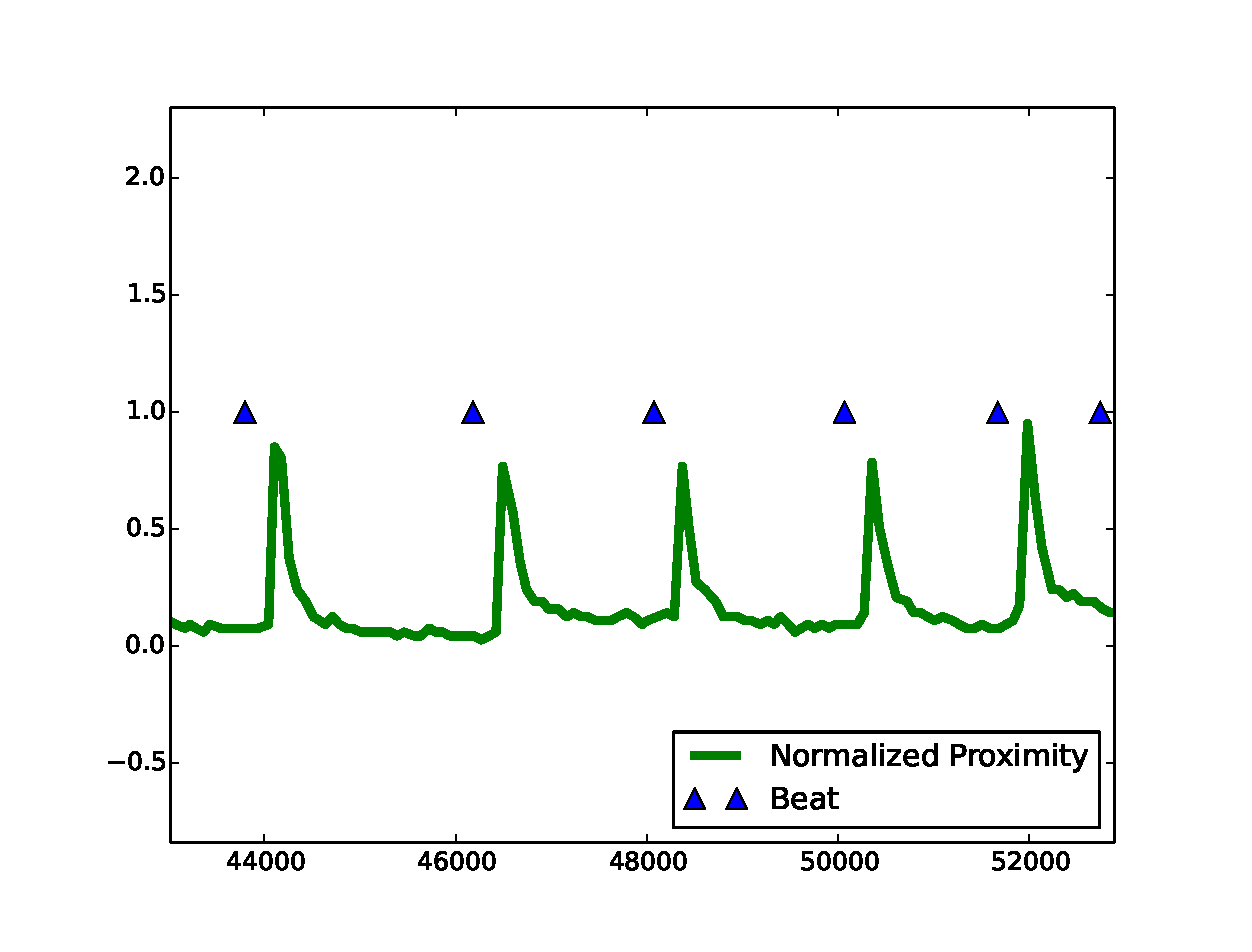
\includegraphics[width=0.75\linewidth]{../figure/sub1_blink_beat} \\
(a)\\
\vspace{-4pt}
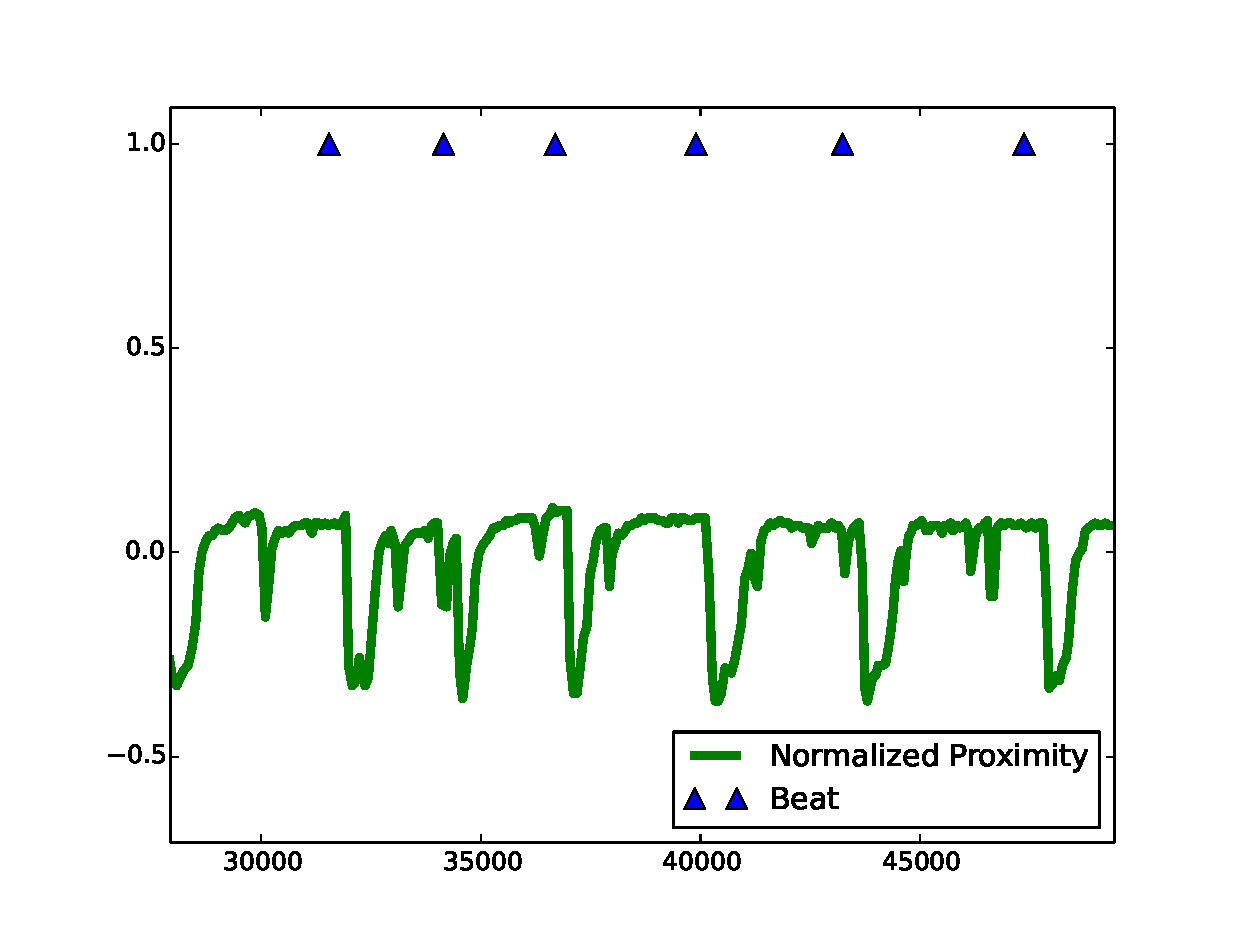
\includegraphics[width=0.75\linewidth]{../figure/sub2_blink_beat} \\
(b)\\
\end{tabular}
    \caption{\label{fig:blink} A person's blinking patterns with respect to music beats are also differentiable.}
\vspace{-6pt}
\end{wrapfigure}
Smart-glass devices typically contain an array of motion sensors such as accelerometer, gyroscope, and inertial measurement unit (IMU). It is only a matter of time that motion sensor chips will be integrated into wearable devices.
This opens up opportunities for multi-modal motion sensing. For example,
accelerometer data can be combined with gyroscope measurements to provide
multi-dimensional head-movement features that can improve the quality of the
inferred signatures. Head movements can also be combined with other body movements to generate
valuable, reliable signatures for authentication. In this project, we plan to explore these opportunities.
%Additionally, head-movement is just one type of body movements, and we can
%investigate other types of body movements as well.


\vspace{4pt}\textbf{Combining Multiple Movement Signatures:} In our preliminary study, we only looked at monitoring head movements for authenticating Google Glass. In reality, there are other types of movements that can be captured by Google Glass for authentication purposes. For example, through a simple test experiment using the Google Glass
infra-red light sensor we observed that the blinking and winking patterns of users in
response to the can be combined with head-movements for better results. *** YZ: Sugang, please include the blinking/winking picture here *** Recent studies have shown that heart beat or pulse can be read by Google Glass~\cite{hernandezbioglass}. In this project, we will also look at whether the pulse information captured by the device can be combined with head movements for more accurate authentication.

The main challenge in combining multiple movement signatures stems from the fact that it is hard to separate their impacts on motion sensor readings (e.g, the fact that a user winks may change the way she moves her head). Hence, it may lead to less accurate authentication results. In this project, we will find ways of handing this challenge, similar to how we propose to authenticate walking users.

\vspace{4pt}\textbf{Combining Accelerometer and Gyroscope:} Many previous studies have looked at combined accelerometer and gyroscope readings in detecting motion contexts such as walking, standing or fall~\cite{mayagoitia2002accelerometer,jovanov2005wireless,li2009accurate,zhu2004real,williamson2001detecting,sabatini2005assessment}. In our preliminary study, however, we find that gyroscope data from Goolge Glass fare very poorly in discriminating users' head movements. The reason is ***
